%%%%%%%%%%%%%%%%%%%%%%%%%%%%%%%%%%%%%%%%%%%%%%%%%%%%%%%%%%%%%%%%%%%%%%%%%%%%%%%%%%%%%%%%%%%%%%%%%%%%%%%%%%%%%%%%%%%%%%%%%%%%%%%%%%%%%
\section{Simulation Results}
\label{sec:simulation_results}

This section presents the results of the proposed control methods.
%
MATLAB Simulink$^\text{{\tiny{\circledR}}}$ models were implemented for the simulation of the dynamic model of a $3$-DOF ISP installed on a vessel and for the implementation of the cascade Super Twisting Control (STC) strategies proposed in \sref{sec:control}.

Joint friction torques were simulated as the sum of Stribeck, Coulomb and viscous friction components, and a saturation of $\pm 12.2 \, Nm$ in each joint motor was considered.
%
The joint encoders and the INS were modeled considering hardware effects such as resolution, bias and noise, and the base motion data
%represented by variables $r_{0}$, $V^{0}_{0}$ and $\dot{V}^{0}_{0}$
were obtained from the simulation of a vessel subject to Jonswap spectrum waves with 200 harmonics, $3$m height, $10$s time period, and acting on the longitudinal axis of the vessel.

\begin{remark}
The presented control methods can be applied to any kind of vehicle or moving base where the ISP is installed, since the quaternion formalism does not suffer from representation singularities and the base dynamics (velocities and accelerations) only affect the overall magnitude of the gains.
\end{remark}

{\renewcommand{\arraystretch}{1.5}%
\begin{table}[!htb]
\caption{Kinematic and dynamic model parameters, in SI units.}
\centering
%\caption{Kinematic and dynamic model parameters.}
\resizebox{\columnwidth}{!}{%
\begin{tabular}{c|ccc|ccc|ccc}
\hline
\multirow{2}{*}{Parameter} & \multicolumn{3}{c|}{$i=1$} & \multicolumn{3}{c|}{$i=2$} & \multicolumn{3}{c}{$i=3$} \\ \cline{2-10}
                           & $x$     & $y$    & $z$     & $x$      & $y$    & $z$    & $x$    & $y$    & $z$      \\ \hline \hline
$p^{i}_{i\bar{i}}$         & 0.006 & 0.023 & 0.326 & -0.094 & 0.006 & 0.059 & 0.336  & 0.006 & -0.023 \\
$p^{i-1}_{i-1\,,i}$ 				 & 0.3   & 0    & 0    & 0      & 0     & 0.436 & -0.254 & 0     & 0      \\
%$h^{i-1}_i$                & 0.0178  & -0.0171 & 0.9997 & -0.0171 & 0.9997 & 0.0174  & 0.9997 & 0.0174 & -0.0175        \\
$I^{\bar{i}}_{\bar{i}}$    & 2.42    & 0.58    & 1.93     & 1.12     & 0.92    & 0.88   & 0.54   & 0.93   &  0.86  \\ \hline
%$h^{i-1}_i$              & \multicolumn{3}{c|}{$z_0$}   & \multicolumn{3}{c|}{$y_0$}  & \multicolumn{3}{c}{$x_0$}    \\ \hline
$m_i$                      & \multicolumn{3}{c|}{18.9}    & \multicolumn{3}{c|}{21}     & \multicolumn{3}{c}{26.5}    \\ \hline
\end{tabular}%
}
\label{table:ISP_parameters}
\end{table}
}
%
\tref{table:ISP_parameters} contains the kinematic and dynamic parameters used in the simulations.
%
The \textit{real} joint axis are considered as $h^{0}_1 \!=\! z_0$, $h^{1}_2 \!=\! y_0$ and $h^{2}_3 \!=\! x_0$. Also, we have $p^3_{3c} = \mat{0.555 & 0 & 0.014}^\mathsf{T}$, and the inertia tensor represented in $\mathbf{E}_{i}$ can be computed from the \textit{Huygens-Steiner theorem} as $I^{i}_{i} = I^{\bar{i}}_{\bar{i}} - m_i \, (\widehat{p}^{i}_{i\bar{i}})^2$.
%
%$p^s_{sc} = \mat{0.405 & 0 & 0.176}^\mathsf{T}$, and $R_{3c} = R_{sc} = \mathbf{I}_3$, where $p^s_{sc}$ and $R_{sc}$ are used only in the direct stabilization case.
%
These parameters were obtained from the mechanical design of a 3-DOF ISP currently being developed by a collaboration among several groups, including the authors laboratory (LEAD/COPPE/UFRJ).

The mass matrices in \eqref{eq:u_sliding} and \eqref{eq:u_sliding_HOSMO} and the Jacobian matrix in \eqref{eq:w_sliding} were computed using 
numerical algorithms, implemented with MATLAB$^\text{{\tiny{\circledR}}}$ mex files.
%\algref{alg:forward_propagation} and \algref{alg:backward_propagation}, implemented with MATLAB$^\text{{\tiny{\circledR}}}$ mex files.
%
The values for the nominal parameters used in control were set as the real values
in Table \ref{table:ISP_parameters} with a percentage of error.
%
The gains for both state and output feedback controllers were set as $\Lambda_1 = \Lambda_2 = 10 \, \mathbf{I}_3$, $\Lambda_3 = \Lambda_4 = 15 \, \mathbf{I}_3$, and the HOSMO gains were chosen as $K_1 = K_2 = K_3 = 15$. These values are sufficient to overcome the magnitude of the disturbances and small enough to avoid chattering effects.
%
The quaternion reference was computed from the roll $\phi_{c}(t)$, pitch $\theta_{c}(t)$ and yaw $\psi_{c}(t)$ (RPY) references for the camera orientation $\eta_{c}(t) = [\, \phi_{c}(t) \,\, \theta_{c}(t) \,\, \psi_{c}(t) \,]^\mathbf{T}$, consisting of unbiased sines with $60^\circ$ of amplitude and $10 \, s$ period.

%%%%%%%%%%%%%%%%%%%%%%%%%%%%%%%%%%%%%%%%%%%%%%%%%%%%%%%%%%%%%%%%%%%%%%%%%%%%%%%%%%%%%%%%%%%%%%%%%%%%%%%%
\subsection{Full State Feedback STC}

Figure \ref{fig:CDC_result1} shows the transient and steady-state response of the state feedback STC in terms of RPY errors for the case of 50\% of parametric error and $5^\circ$ degrees of axis misalignment in the computation of the Jacobian matrix. 
%
%\vspace{-2.5mm}
\begin{figure}[!htpb]
\centering
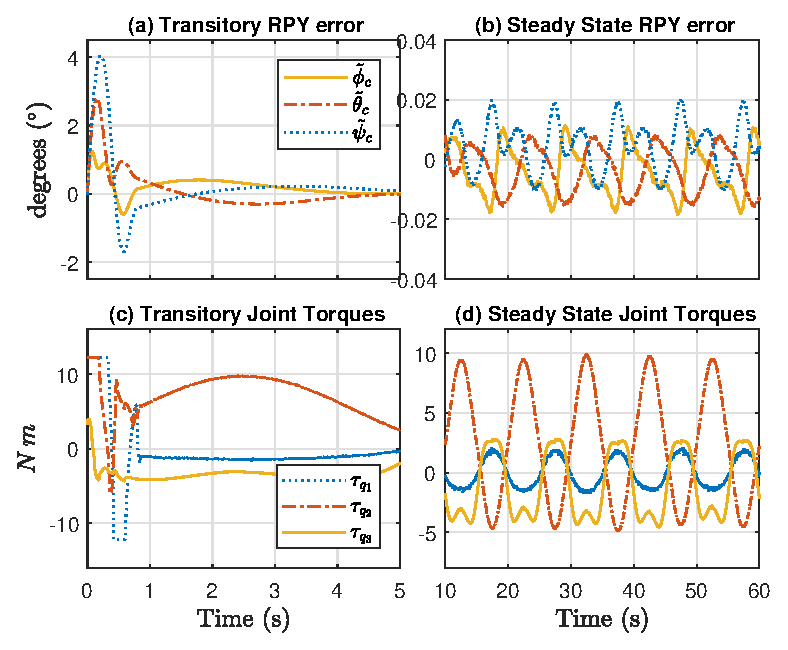
\includegraphics[width=1.0\columnwidth]{results/CDC_result1}
\caption{Response for state feedback STC controller with 50\% of parametric error and $5^\circ$ degrees of axis misalignment.}
\label{fig:CDC_result1}
\end{figure}
%
Both stabilization and tracking controllers achieve SOSM in less than $2\,s$, with sliding accuracy on $s_x$ and $s_y$ approximately equal to $10^{-4} \, rad/s$ and $10^{-5}$, respectively.
%
The RPY jitter converges to a small region of $0.02^{\circ}$ in approximately $10\,s$ due to the chosen dynamics for the outer sliding surface.

%Figure \ref{fig:CDC_result2} shows the response for the case of 50\% of parametric error and a first-order linear actuator dynamics with $25 \, ms$ of rising time to simulate the driver dynamics. Clearly, performance is strongly affected in the presence of unmodeled dynamics, with sliding accuracy exceeding $10^0 \, rad/s$ and $10^{-1}$ for $s_x$ and $s_y$. The torque chattering is higher as well, with chattering period of approximately $0.16\,s$ in the steady-state response.

%%%%%%%%%%%%%%%%%%%%%%%%%%%%%%%%%%%%%%%%%%%%%%%%%%%%%%%%%%%%%%%%%%%%%%%%%%%%%%%%%%%%%%%%%%%%%%%%%%%%%%%%%%%%%%%%%%%%%%%%%%%%%%%%%%%%%
\subsection{Output Feedback STC + HOSMO}

Figure \ref{fig:CDC_result2} shows the transient and steady-state response of the of the output feedback STC, in the same conditions as before. 
%
%\vspace{-2.5mm}
\begin{figure}[!htpb]
\centering
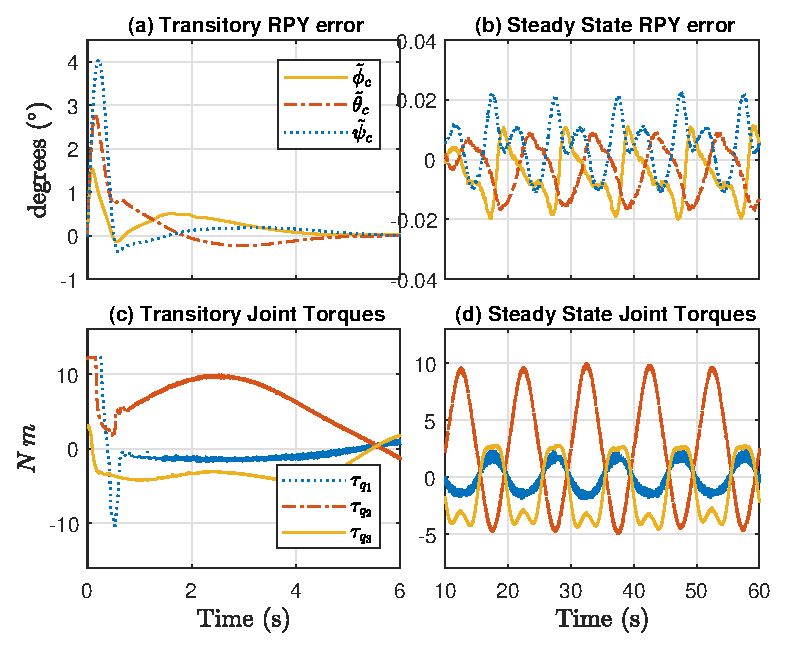
\includegraphics[width=0.95\columnwidth]{results/CDC_result2}
\caption{Response for output feedback STC controller with 50\% of parametric error and $5^\circ$ degrees of axis misalignment.}
\label{fig:CDC_result2}
\end{figure}
%
The transient and performance remains practically the same, with a very small increase in the RPY jitter and in the control chattering.
%
This is due to the presence of the term dependent multiplying $K_2$ in \eqref{eq:u_sliding_HOSMO}.

Figure \ref{fig:CDC_result3} shows the HOSMO estimation errors of the output feedback STC scheme. 
%
%\vspace{-2.5mm}
\begin{figure}[!htpb]
\centering
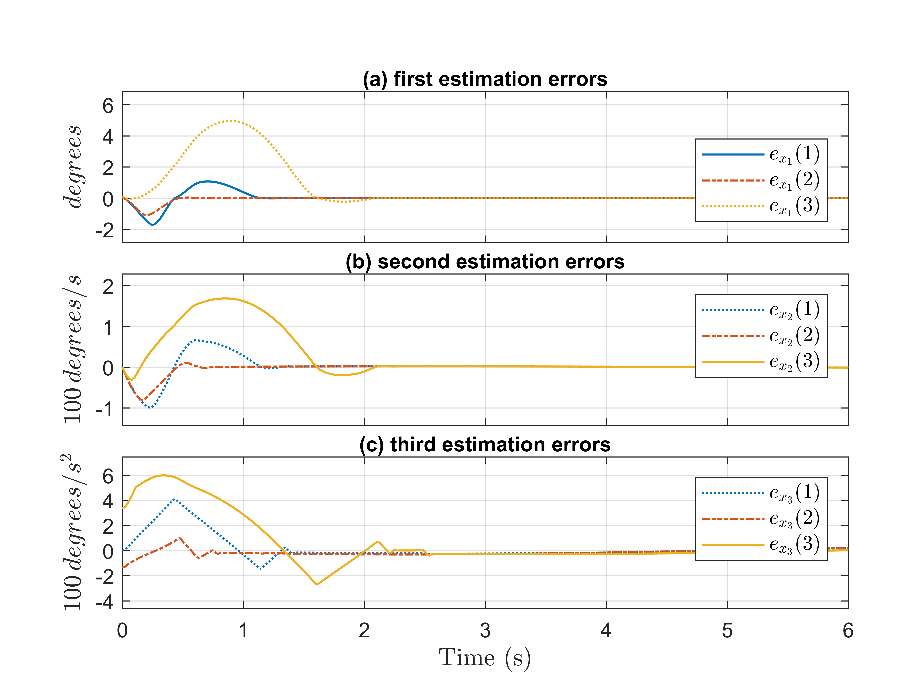
\includegraphics[width=1.0\columnwidth]{results/CDC_result3}
\caption{HOSMO estimation errors for output feedback STC controller with 50\% of parametric error.}
\label{fig:CDC_result3}
\end{figure}
%
Note that finite-time convergence is achieved in approximately $3\,s$, even in the presence of sensor noise and 50\% of parametric error in $\widehat{M}_{qq}$ used in \eqref{eq:x_HOSMO}.
%


